\section{Measured forbidden components}
\begin{table}[htbp]\centering
\begin{tabular}{rrrrr}
\toprule
Reference / $^\circ$C & Candidates & Supported & $r_d$ RMS & $r_q$ RMS\\
\midrule
30 & 158 & 142 & 2.873 & 2.184 \\
70 & 158 & 144 & 2.477 & 2.127 \\
\bottomrule
\end{tabular}

\caption{Mirror-interpolation demonstration. Residual RMS is in mWb; support
counts describe positive-q representatives, not independent sensor trials.}
\end{table}
The observed forbidden components are on the scale of a few mWb. Their thermal
reference dependence is descriptive: a rotor reference does not establish
winding equilibrium or identify an ohmic cause. Some mirror arguments lie
outside the measured hull and are excluded instead of extrapolated.
\begin{figure}[htbp]\centering
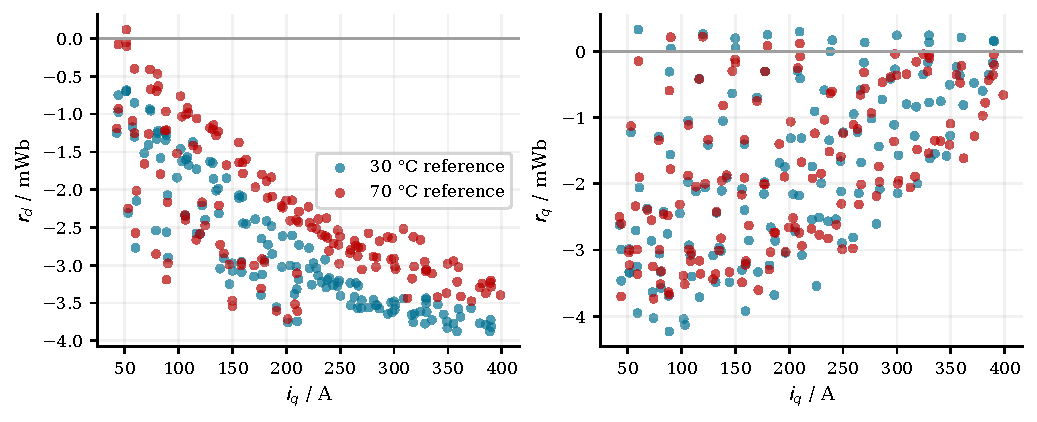
\includegraphics[width=\textwidth]{figures/real_projection.pdf}
\caption{Raw forbidden d-odd and q-even components on supported measured-current
mirrors. Separate thermal references are shown with the common visual palette.}
\label{fig:real-projection}\end{figure}
At each retained pair the projected values satisfy parity to roundoff.
That is a check of the operator, not experimental proof of a corrected machine.
An allowed-parity perturbation survives unchanged, however large it is.
